\documentclass[tikz,border=6pt]{standalone}
% Shared figure style for the Space Data Network whitepapers.
\usepackage{lmodern}
\usepackage[T1]{fontenc}
\usepackage{xcolor}
\usetikzlibrary{arrows.meta,positioning,calc,fit,backgrounds,matrix}
\hyphenpenalty=10000\exhyphenpenalty=10000
\definecolor{ink}{HTML}{1F2328}
\definecolor{rule}{HTML}{57606A}
\definecolor{panel}{HTML}{F3F4F6}
\definecolor{accent}{HTML}{D4880F}
\tikzset{
  every picture/.style={line width=0.6pt, draw=ink, text=ink, font=\small},
  box/.style={draw=ink, fill=panel, rounded corners=2pt, align=center, inner sep=5pt},
  plain/.style={draw=ink, fill=white, rounded corners=2pt, align=center, inner sep=5pt},
  title/.style={font=\bfseries\small},
  where/.style={font=\scriptsize\itshape, text=rule},
  note/.style={font=\footnotesize\itshape, text=rule},
  flow/.style={-{Stealth[length=2.2mm]}, draw=rule},
}

\begin{document}
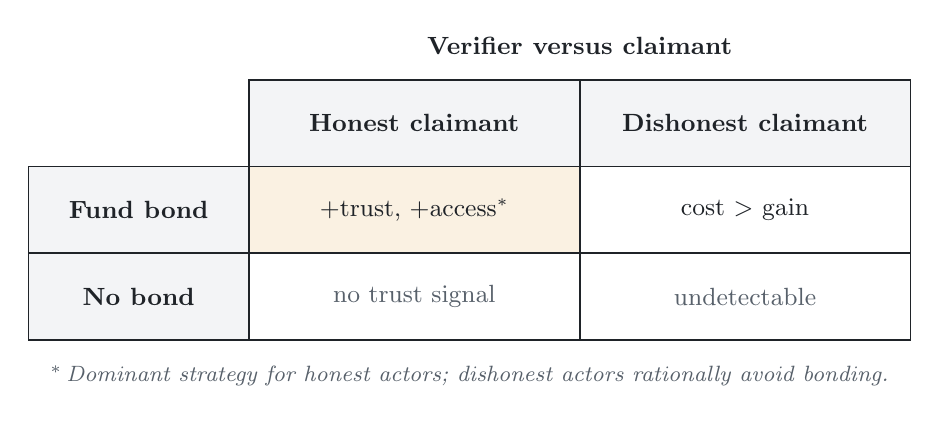
\begin{tikzpicture}[x=1mm, y=1mm, c/.style={align=center, font=\small}]
\def\w{42}\def\h{11}\def\r{28}
% header fills
\fill[panel] (\r,0) rectangle (\r+2*\w,\h);
\fill[panel] (0,-2*\h) rectangle (\r,0);
\fill[accent!12] (\r,-\h) rectangle (\r+\w,0);
% grid
\draw (\r,\h) rectangle (\r+2*\w,-2*\h);
\draw (0,0) rectangle (\r,-2*\h);
\draw (\r,0) -- (\r+2*\w,0) (0,-\h) -- (\r+2*\w,-\h) (\r+\w,\h) -- (\r+\w,-2*\h);
\node[c, font=\bfseries\small] at (\r+0.5*\w,0.5*\h) {Honest claimant};
\node[c, font=\bfseries\small] at (\r+1.5*\w,0.5*\h) {Dishonest claimant};
\node[c, font=\bfseries\small] at (0.5*\r,-0.5*\h) {Fund bond};
\node[c, font=\bfseries\small] at (0.5*\r,-1.5*\h) {No bond};
\node[c] at (\r+0.5*\w,-0.5*\h) {$+$trust, $+$access$^{*}$};
\node[c] at (\r+1.5*\w,-0.5*\h) {cost $>$ gain};
\node[c, text=rule] at (\r+0.5*\w,-1.5*\h) {no trust signal};
\node[c, text=rule] at (\r+1.5*\w,-1.5*\h) {undetectable};
\node[font=\bfseries\small, anchor=south] at (\r+\w,\h+2) {Verifier versus claimant};
\node[note, anchor=north] at (0.5*\r+\w,-2*\h-2) {$^{*}$\,Dominant strategy for honest actors; dishonest actors rationally avoid bonding.};
\end{tikzpicture}
\end{document}
